\documentclass[class=minimal,border=0pt]{standalone}
\usepackage{tikz}
\usepackage{amsmath}

\usetikzlibrary{%
  arrows,
  calc
}
\usetikzlibrary{decorations.markings}
\usetikzlibrary{shapes.misc}

\begin{document}
  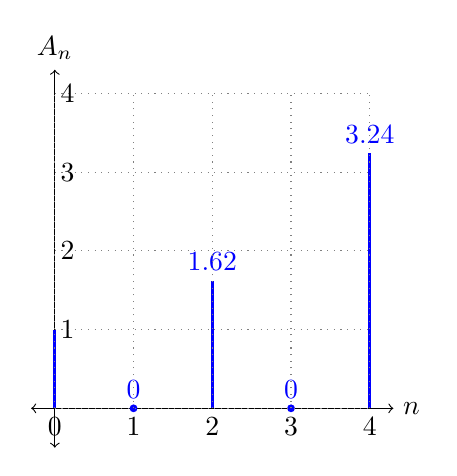
\begin{tikzpicture}[yscale=1, xscale=1]
    \draw[<->] (-0.3,0) -- (4.3,0) node[right] {$n$};
    \draw[<->] (0,-0.5) -- (0,4.3) node[above] {$A_n$};
    

    \draw[-,line width = 1pt, blue] (0,0) -- (0,1);
     \node at (1,0) [circle,fill,inner sep=1pt,blue]{};
      \draw (1,0) node[blue,above] {$0$};
    \draw[-,line width = 1pt, blue] (2,0) -- (2,1.62);
     \draw (2,1.62) node[blue,above] {$1.62$};
    \node at (3,0) [circle,fill,inner sep=1pt,blue]{};
     \draw (3,0) node[blue,above] {$0$};
    \draw[-,line width = 1pt, blue] (4,0) -- (4,3.24);
     \draw (4,3.24) node[blue,above] {$3.24$};
   
 
    \draw (0,0) node[below] {$0$};
    \draw (1,0) node[below] {$1$};
    \draw (2,0) node[below] {$2$};
    \draw (3,0) node[below] {$3$}; 
    \draw (4,0) node[below] {$4$};

    \draw (-0.05,4) node[right] {$4$};
	\draw (-0.05,3) node[right] {$3$};
    \draw (-0.05,2) node[right] {$2$};
    \draw (-0.05,1) node[right] {$1$};
    
    
    

    \draw[dotted,step=1cm,color=gray, thin] (0,0) grid (4,4);

  \end{tikzpicture}

\end{document}